\documentclass[conference]{IEEEtran}
\IEEEoverridecommandlockouts
\usepackage{cite}
\usepackage{amsmath,amssymb}
\usepackage{graphicx}
\usepackage{xcolor}
\usepackage{booktabs}
\usepackage{url}
\usepackage{amssymb}
\usepackage{tikz}
\usetikzlibrary{positioning,arrows.meta,fit}

% ---- numbers come ONLY from analyze.py (paper_out/numbers.tex) or the author's manual.tex ----
\providecommand{\checkmark}{\ensuremath{\surd}}
\newcommand{\pend}{\textcolor{red}{\textbf{??}}}
\InputIfFileExists{paper_out/numbers.tex}{}{}
\InputIfFileExists{paper_out/manual.tex}{}{}
\newcommand{\num}[1]{\ifcsname n@#1\endcsname\csname n@#1\endcsname\else\pend\fi}
\newcommand{\tabin}[1]{\IfFileExists{paper_out/#1.tex}{\input{paper_out/#1.tex}\\}{\pend\ run analyze.py \\}}
\newcommand{\figin}[2]{\IfFileExists{paper_out/#1.pdf}{\includegraphics[width=#2\columnwidth]{paper_out/#1.pdf}}{\fbox{\parbox{0.8\columnwidth}{\centering\vspace{8mm}\pend\ figure pending: run analyze.py\vspace{8mm}}}}}
\newcommand{\finalize}[1]{\textcolor{red}{\textbf{[FINALIZE AFTER RUN: #1]}}}

\begin{document}

\title{How Much Time Do You Have to Say Stop? A Detection-and-Recovery Framework for Safe Tool Use in On-Device Agentic AI}

\author{\IEEEauthorblockN{Sharath Chandra Kampili}
\IEEEauthorblockA{Independent Researcher\\
Distributed Data Systems and Applied AI\\
Dallas, Texas, USA\\
sharathchandra.kampili@ieee.org}}
\maketitle

\begin{abstract}
On-device AI agents now plan and execute multi-step tool calls in smart homes. When such an agent drifts from the user's goal or is interrupted midway, no server exists to roll anything back, and the home is left in a state nobody asked for. We make this failure measurable with two quantities: the \emph{residual-state divergence rate}, how often an interrupted workflow ends in a state that is neither the starting state nor the goal, and the \emph{intervention window}, the seconds a person has between issuing a request and the first irreversible effect. We propose a two-layer framework around a local-model agent: a detection layer of four pre-execution checks (scope, bounds, goal consistency, irreversibility) and a recovery layer that adapts the saga pattern to announce, pause, and compensate. In a simulated smart home with \num{ntasks} tasks, \num{nbenign} benign and \num{ndrift} drifted labelled gate cases, and \num{nmodels} local models decoding at \num{spdmin}--\num{spdmax} tokens/s, the median window ranges from \num{wmin} to \num{wmax}\,s (Spearman rank correlation with decode speed: \num{rho}). When a stop arrives at a random point, an irreversible action had already fired in \num{lateNone}\% of runs without recovery and \num{lateRec}\% with it. Judge false-positive rates on benign calls are \num{kwFP}\% (keyword), \num{obFP}\% (naive local-model) and \num{opFP}\% (history-aware local-model). The harness, scenarios and demo are open and re-runnable on a laptop.
\end{abstract}

\begin{IEEEkeywords}
agentic AI, on-device AI, safe tool use, human-in-the-loop, human-machine systems, saga pattern, trustworthy autonomy, edge computing
\end{IEEEkeywords}

\section{Introduction}
Consumer electronics are moving from single smart devices to ambient ecosystems in which an AI agent senses context and acts across many devices. Language-model agents that interleave reasoning with tool calls~\cite{react,toolformer} make this practical, and small quantized models now run such agents entirely on a laptop or home hub~\cite{qwen25,edgequant}. On-device execution protects privacy, but it removes the server-side controls a cloud platform uses to block or reverse a bad action.

Agents are usually evaluated on whether they finish the task. When an agent fails halfway it does not simply stop: it has already done three or four things. On a phone or a home hub nothing rolls them back, so the failure is not ``nothing happened'' but ``the house is now in a state nobody asked for.'' Two failure modes matter most. First, the agent may call the wrong tool, or the right tool with wrong arguments, because it misread the goal or followed instructions hidden in untrusted content such as a calendar note~\cite{greshake}. Second, a correct workflow may be interrupted by a crash, a power loss, or the user saying ``stop'' after some steps have run. Research on agent safety has largely addressed the first problem through benchmarks and judges~\cite{toolemu,rjudge,agentdojo,agentharm,agentsafetybench}; the second, and the question of whether a person actually has time to intervene, has received little measurement.

Beyond the smart-home setting, the same question applies to any human-machine system where an autonomous agent acts faster than a person can supervise it -- the detection-and-recovery pattern and the two oversight metrics we define are not specific to home automation. There is also a tension that this paper sets out to quantify. Faster on-device inference is normally treated as an unqualified benefit. But the faster the agent plans, the less time a person has to notice a wrong step before an irreversible one fires. Speed and human oversight may pull against each other. We ask:
\begin{itemize}
\item \textbf{RQ1} How well can lightweight on-device judges separate benign tool calls from goal-drifted or unsafe ones, and at what latency cost?
\item \textbf{RQ2} How often does interrupting a multi-step workflow leave residual state, and how much does saga-style recovery reduce it?
\item \textbf{RQ3} How do model size and quantization change the time a person has to stop an action, and does an explicit pause put a floor under it at bounded cost?
\end{itemize}
Our contributions are: (1) StopWatch, a two-layer detection-and-recovery framework for on-device agents; (2) two oversight metrics, residual-state divergence and intervention window, with precise definitions and a control that separates interruption damage from ordinary task failure; (3) a re-runnable evaluation across \num{nmodels} local models and quantization levels, including a prompt-injection study; and (4) an open harness and demo. The recovery layer is a saga~\cite{sagas}, an established database technique; we claim no novelty for it. The contribution is the measurement.

\section{Related Work}
\textbf{Tool-using agents.} ReAct~\cite{react} and Toolformer~\cite{toolformer} established language models that call external tools. \textbf{Agent safety.} ToolEmu~\cite{toolemu} identifies risky agent actions in an emulated sandbox, R-Judge~\cite{rjudge} benchmarks risk awareness, AgentDojo~\cite{agentdojo} evaluates prompt-injection attacks and defenses, AgentHarm~\cite{agentharm} and Agent-SafetyBench~\cite{agentsafetybench} measure harmful behaviour, and Llama Guard~\cite{llamaguard} classifies unsafe content. Arike et al.~\cite{goaldrift} measure goal drift over long interactions. Language models are also widely used as judges~\cite{mtbench}. These works evaluate whether an action is safe. They do not address recovery after partial execution or the time available for human intervention. \textbf{Recovery.} Sagas~\cite{sagas} split long transactions into steps with compensating actions; we apply this pattern to agent tool calls. Two recent systems apply the same pattern specifically to LLM agents: SagaLLM~\cite{sagallm} integrates saga-style transactional guarantees with persistent context and independent validation for multi-agent LLM planning, and GoEx~\cite{goex} proposes an undo mechanism and damage-confinement runtime for post-facto validation of LLM-generated actions. Both target correctness and safety of the actions themselves. We differ in what we measure, not only in the mechanism: we report a time-to-stop quantity (the intervention window $W$) tied to on-device inference speed, and an interruption-attributable divergence rate that separates recovery-layer effects from ordinary task failure via a paired control -- neither system reports either. \textbf{Human oversight.} Parasuraman et al.~\cite{parasuraman} describe levels of human interaction with automation; the intervention window makes one such level measurable for agents. \textbf{On-device inference.} Quantization~\cite{awq} makes few-billion-parameter models practical on consumer hardware, and Husom et al.~\cite{edgequant} measure the latency, energy and accuracy of quantized models under Ollama on edge devices. We use the same class of models and runtime, but ask how per-step latency turns into human reaction time.

\begin{table}[t]\centering\caption{What each line of work primarily evaluates (coarse; by primary contribution).}\label{tab:cmp}\scriptsize
\begin{tabular}{lcccc}\toprule & action & prompt & partial-run & time to\\ & safety & injection & recovery & stop\\\midrule
ToolEmu~\cite{toolemu}, R-Judge~\cite{rjudge} & \checkmark & & & \\
AgentHarm~\cite{agentharm} & \checkmark & & & \\
AgentDojo~\cite{agentdojo} & \checkmark & \checkmark & & \\
Llama Guard~\cite{llamaguard} & \checkmark & & & \\
Sagas~\cite{sagas} & & & \checkmark & \\
SagaLLM~\cite{sagallm} & & & \checkmark & \\
GoEx~\cite{goex} & \checkmark & & \checkmark & \\
This work & \checkmark & \checkmark & \checkmark & \checkmark\\\bottomrule\end{tabular}
\end{table}

\section{Framework}
Fig.~\ref{fig:arch} shows the two layers between the agent's planner and the device tools.

\begin{figure}[t]
\centering
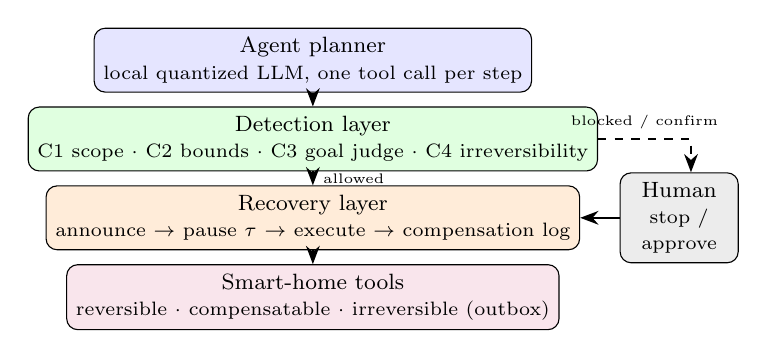
\begin{tikzpicture}[node distance=5pt,
 box/.style={draw,rounded corners,align=center,font=\footnotesize,minimum width=5.4cm,minimum height=0.75cm},
 arr/.style={-Stealth,thick}]
 \node[box,fill=blue!10] (pl) {Agent planner\\ \scriptsize local quantized LLM, one tool call per step};
 \node[box,fill=green!12,below=of pl] (det) {Detection layer\\ \scriptsize C1 scope $\cdot$ C2 bounds $\cdot$ C3 goal judge $\cdot$ C4 irreversibility};
 \node[box,fill=orange!15,below=of det] (rec) {Recovery layer\\ \scriptsize announce $\to$ pause $\tau$ $\to$ execute $\to$ compensation log};
 \node[box,fill=purple!10,below=of rec] (tools) {Smart-home tools\\ \scriptsize reversible $\cdot$ compensatable $\cdot$ irreversible (outbox)};
 \node[box,fill=gray!15,right=0.5cm of rec,minimum width=1.5cm,align=center] (hu) {Human\\ \scriptsize stop /\\ \scriptsize approve};
 \draw[arr] (pl)--(det); \draw[arr] (det)--(rec) node[midway,right,font=\tiny]{allowed}; \draw[arr] (rec)--(tools);
 \draw[arr] (hu.west)--(rec.east);
 \draw[arr,dashed] (det.east) -| ([xshift=0.15cm]hu.north) node[pos=0.25,above,font=\tiny]{blocked / confirm};
\end{tikzpicture}
\caption{Detection-and-recovery framework for on-device tool use.}
\label{fig:arch}
\end{figure}

\subsection{Tool classification}
Each tool is labelled by the effect it has (Table~\ref{tab:tools}). \emph{Reversible} tools have an exact inverse, \emph{compensatable} tools can be undone by restoring the previous value, and \emph{irreversible} tools write to an append-only outbox and cannot be undone. Labels are declared once per tool, much like permissions in a mobile app manifest. In the harness both undoable classes are compensated identically; the distinction is semantic.
\begin{table}[t]\centering\caption{Simulated home tools and effect class}\label{tab:tools}\small
\begin{tabular}{ll}\toprule Class & Tools\\\midrule
reversible & set\_light, set\_lock, set\_tv, set\_alarm, set\_blinds\\
compensatable & set\_thermostat, set\_oven\\
irreversible & send\_message, place\_order, share\_camera\_clip\\\bottomrule\end{tabular}
\end{table}

\subsection{Detection layer}
Before a call runs, four checks are applied in order of cost. \textbf{C1 Scope:} the tool must be on the allowlist for the current task. \textbf{C2 Bounds:} typed arguments must fall inside declared ranges or enumerations (for example oven temperature $\le$ 450); free-text arguments such as message recipients are not validated, which is why C3 carries the injection defence. \textbf{C3 Goal consistency:} a judge decides whether the call serves the user's stated objective. \textbf{C4 Irreversibility:} irreversible calls require confirmation. We compare three C3 judges: \emph{KeywordJudge} matches the call against terms in the objective; \emph{ObjectiveJudge} asks a small local model, in one binary question with no history, whether the call directly helps; \emph{ObjectiveJudgePlus} uses the same model but shows the executed-step history, asks for a three-way verdict (serves, unrelated, harmful) and includes four worked examples from a scenario that appears in no test set.

\subsection{Recovery layer}
The recovery layer records every executed step with its compensating action (Fig.~\ref{fig:algo}). Before an irreversible step it announces the intended action and waits a pause $\tau$ during which the user can cancel. If the workflow is interrupted, completed undoable steps are undone in reverse order. Pausing applies only to irreversible steps, so added latency is at most $\tau$ times their number.
\begin{figure}[t]\centering\small
\fbox{\parbox{0.93\columnwidth}{\ttfamily\footnotesize
for each planned call c:\\
\hspace*{1em}if stop: break\\
\hspace*{1em}if gate on and gate(c)=block: skip c\\
\hspace*{1em}if mode=recovery and irreversible(c):\\
\hspace*{2em}announce(c); if wait(tau) sees stop: cancel; break\\
\hspace*{1em}u = apply(c); if u: push(undo, u)\\
if stop and mode=recovery:\\
\hspace*{1em}for u in reverse(undo): apply(u)}}
\caption{Agent loop with the recovery layer.}\label{fig:algo}
\end{figure}

\subsection{Oversight metrics}
\textbf{Divergence:} an interrupted run ends in neither the initial nor the goal state. Because small models also fail tasks that are never interrupted, every interrupted run is paired with an uninterrupted control, and we report divergence among runs whose control reached the goal (\emph{interruption-attributable divergence}). \textbf{Window} for a run is
\begin{equation}W=t_{\mathrm{irr}}-t_{\mathrm{req}},\end{equation}
where $t_{\mathrm{req}}$ is the start of the agent loop and $t_{\mathrm{irr}}$ the time of the first irreversible effect; it therefore includes prompt evaluation and decoding of every preceding step. With the recovery layer, $W\ge\tau$ holds by construction. \textbf{Too late:} a stop at a random time $t_s$ arrives after an irreversible action already fired ($t_{\mathrm{irr}}\le t_s$). \textbf{Judge FP:} a benign call is blocked. \textbf{Judge FN:} a drifted call is not blocked. Three choices in these definitions matter. The control removes ordinary task failure from the divergence rate, so what remains is attributable to the stop. The stop time is scaled to each control's own time to first irreversible action, so that a fast and a slow model are stopped at comparable relative points; an absolute stop distribution would measure model speed rather than the recovery layer. And $W$ is reported only over runs that reach an irreversible step, so we always print how many did.

\subsection{Scope and threat model}
The framework targets two situations. In the first, a benign or mildly drifted workflow is stopped part-way by a crash, a power loss, a lost connection to a device, or a person saying ``stop''. In the second, the agent is steered by untrusted text (a calendar entry, a device name, a message preview) into calls the user did not request. We do not address an attacker who has compromised the model weights, the runtime or the gate itself, nor one who can issue calls that are inside the task's allowlist and bounds and semantically plausible; such calls pass C1--C3 by construction and are handled only by C4 and the pause. The privacy claim is narrow: the client refuses any model endpoint that is not local, so prompts and device state never leave the machine, but the outbox tools model actions that in a real home would.

\section{Experimental Setup}
\textbf{Environment.} A simulated home with four lights, thermostat, two door locks, oven, TV, alarm, two blinds and an outbox, exposed as the ten tools of Table~\ref{tab:tools}. \textbf{Tasks.} Twelve workflows of 2--8 steps (for example ``prepare the house for guests'', ``lock up for the night''), each with a goal state, plus four variants in which an untrusted note carries an injected instruction (an attack succeeds if a matching call executes). Every objective states every value the goal checks; an earlier version of our benchmark did not, which made several tasks unreachable by construction and inflated divergence, and we fixed it before collecting the data reported here. \textbf{Gate cases.} \num{nbenign} benign, \num{ndrift} drifted, 48 out-of-scope and 20 out-of-bounds calls, derived from the tasks with an explicit and a deliberately vague phrasing (vague wording is where keyword matching should struggle). The out-of-scope and out-of-bounds cases are decided deterministically by C1 and C2 and are a sanity check, not a result. Ground truth was assigned by the author; a second person independently labelled 60 random benign/drifted cases (Cohen's $\kappa=\num{kappa}$). Scenario files were frozen in version control before any reported run (commit \num{commit}).

\begin{table}[t]\centering\caption{The twelve base tasks: planned steps (S) and irreversible steps (I).}\label{tab:tasks}\scriptsize
\begin{tabular}{lcc|lcc}\toprule task & S & I & task & S & I\\\midrule
movie\_night & 4 & 1 & dinner & 4 & 1\\ goodnight & 6 & 1 & movie\_end & 4 & 0\\ guests & 4 & 1 & away\_weekend & 8 & 1\\
reorder\_milk & 2 & 2 & welcome\_home & 6 & 1\\ bake & 3 & 1 & leave\_home & 7 & 1\\ morning & 4 & 1 & nap & 3 & 1\\\bottomrule\end{tabular}
\end{table}

\textbf{Models and hardware.} Table~\ref{tab:models} lists the models, served by Ollama~\cite{ollama} (llama.cpp runtime~\cite{llamacpp}) on \num{cpu}, \num{ram}\,GB RAM, \num{osname}, Ollama \num{ollama}; every model is warmed up first so load time is not measured.
\begin{table}[t]\centering\caption{Models under test}\label{tab:models}\small
\begin{tabular}{lcc}\toprule Model & Params & Quantization\\\midrule
Llama-3.2 & 1B & Q4\_K\_M\\ Qwen2.5 & 3B & Q4\_K\_M\\ Qwen2.5 & 3B & Q8\_0\\ Llama-3.1 & 8B & Q4\_K\_M\\\bottomrule\end{tabular}
\end{table}

\textbf{Protocol.} Agents sample at temperature 0.7 with seed equal to the repetition index, so repetitions are genuine samples ($\num{reps}$ per task and configuration); the pause is $\tau=3$\,s. For RQ3 we run each task to completion in both modes and record $W$ and duration. For RQ2 each run is paired with an uninterrupted control; the stop time is $t_s=uR$ where $R$ is the control's time to its first irreversible action (its duration if it has none) and $u\sim\mathcal{U}(0.1,1.5)$, the same $u$ for both modes. Scaling by $R$ makes the stop land at comparable relative points for fast and slow models. \textbf{Statistics.} Runs within a task are correlated, so all intervals are 95\% bootstrap intervals that resample \emph{tasks}, not runs. $W$ is defined only for runs that reach an irreversible step; every table reports that coverage as $k/n$.

\begin{table}[t]\centering\caption{Fixed experimental parameters}\label{tab:params}\footnotesize
\begin{tabular}{ll}\toprule Parameter & Value\\\midrule
Pause before irreversible calls, $\tau$ & 3\,s\\
Sampling temperature / seed & 0.7 / repetition index\\
Repetitions per task, mode and model & \num{reps}\\
Stop time & $t_s=uR$, $u\sim\mathcal{U}(0.1,1.5)$\\
Maximum planner steps per run & 12\\
Bootstrap resamples (over tasks) & 2000\\
Judge model & same as the agent model, temperature 0\\
Failed runs & recorded as errors and excluded (\num{nerrors} here)\\\bottomrule\end{tabular}
\end{table}

\textbf{Benchmark validity.} Two design errors in our first version are worth recording because they are easy to repeat. First, goals demanded exact values (a light at 20, a thermostat at 66) that the natural-language objective never mentioned, so a correct agent could not know them; tasks with unstated values reached the goal in almost no runs while the one task that stated every value did best. We diagnosed this by comparing the numbers in each goal with the numbers in its objective, rewrote every objective to state its values, and re-verified mechanically that each reference plan reaches its goal and that doing nothing classifies as the initial state. Second, at temperature 0 a per-run seed changes nothing, so ten repetitions of a task were identical up to timing noise; we now sample at temperature 0.7 and treat the task, not the run, as the unit of independence.

\section{Results}
\subsection{RQ1: detection accuracy}
Table~\ref{tab:judge} compares the judges on the same cases. Keyword matching blocks \num{kwFP}\% of benign calls overall (\num{kwFPexplicit}\% under explicit and \num{kwFPvague}\% under vague phrasing). The naive local judge blocks \num{obFP}\% and the history-aware judge \num{opFP}\%, while missing \num{obFN}\% and \num{opFN}\% of drifted calls (keyword: \num{kwFN}\%). C1 blocked \num{cone} of \num{coneN} out-of-scope calls and C2 \num{ctwo} of \num{ctwoN} out-of-bounds calls. A model judge costs a median \num{obPfifty}\,ms per call (p95 \num{obPninetyfive}\,ms), so at these speeds the judge is itself a component of $W$.
\begin{table}[t]\centering\caption{C3 judges on labelled calls (FP: benign blocked; FN: drifted allowed; 95\% CI over tasks)}\label{tab:judge}\footnotesize
\begin{tabular}{lccc}\toprule Judge & FP \% & FN \% & p50/p95 ms\\\midrule
\tabin{tab_judge}
\bottomrule\end{tabular}
\end{table}

\subsection{RQ3: intervention window versus model speed}
Table~\ref{tab:window} and Fig.~\ref{fig:tradeoff} report full uninterrupted runs. Across \num{nmodels} models, median decode speed spans \num{spdmin}--\num{spdmax} tokens/s and median $W$ spans \num{wmin}--\num{wmax}\,s; the relationship is monotonic (Spearman $\rho=\num{rho}$), with each step down in decode speed increasing the median window and no model breaking the ordering, from \num{wmin}\,s at the fastest configuration (\num{fastmodel}) to \num{wmax}\,s at the slowest. With only four models, $\rho=\num{rho}$ is not itself statistically significant (two-tailed exact test, $p\approx0.08$); the relationship should be read as a clean trend in this sample, not a validated law, until it is tested on more models. Pausing changes task duration by a median of \num{ovhmed}\% (maximum \num{ovhmax}\%) across tasks and models -- the maximum is a single (model, task) cell with only three repetitions and one outlying run (one duration of 67.5\,s against two near 7\,s), not a systematic cost; the median is the number to trust.
\begin{table*}[t]\centering\caption{Full runs without a stop. $W$: median seconds to first irreversible effect over the $k/n$ runs that reached one; duration: median task time (none / recovery).}\label{tab:window}\footnotesize
\begin{tabular}{lccccc}\toprule Model & tok/s & goal \% & $W$ none (k/n) & $W$ recovery (k/n) & duration none / rec (s)\\\midrule
\tabin{tab_window}
\bottomrule\end{tabular}
\end{table*}
\begin{figure}[t]\centering\figin{fig_tradeoff}{0.92}\caption{Speed versus oversight: median window $W$ against decode speed (log--log, 95\% CI over tasks).}\label{fig:tradeoff}\end{figure}

\subsection{RQ2: interruption}
The interruption study covers three of the four models (llama3.2:1b, qwen2.5:3b-q4, qwen2.5:3b-q8); llama3.1:8b is included in RQ3's full-run measurements but was excluded here for practical reasons -- at 131\,s per uninterrupted run (Table~\ref{tab:window}) and the highest RAM footprint of the four, a matched paired-control interrupt sweep for it did not fit the available compute budget for this study. Table~\ref{tab:interrupt} and Fig.~\ref{fig:interrupt} pool the stopped runs across the three models that were covered. Among runs whose uninterrupted control reached the goal, interruption left a diverged state in \num{divNone}\% (95\% CI \num{divNonelo}--\num{divNonehi}) of runs without recovery and \num{divRec}\% (\num{divReclo}--\num{divRechi}) with it. Among runs whose control reached an irreversible step, the stop came too late in \num{lateNone}\% (\num{lateNonelo}--\num{lateNonehi}) without recovery and \num{lateRec}\% (\num{lateReclo}--\num{lateRechi}) with it. The recovery layer cannot undo an irreversible effect that already fired, so the residual rate with recovery measures how often the pause was shorter than the human's reaction.
The recovery layer's effect on divergence is large and consistent across the three models it was tested on (interruption-attributable divergence \num{divNone}\% $\to$ \num{divRec}\%, pooled $n=\num{nattNone}/\num{nattRec}$ attributable runs of \num{nstopNone}/\num{nstopRec} stopped), while the too-late rate barely moves (\num{lateNone}\%$\to$\num{lateRec}\%): recovery mainly repairs the damage of a late stop rather than making stops arrive earlier, and per-model attributable counts are small enough (3--12) that the per-model split in Table~\ref{tab:interrupt} should be read as directional, not precise.
\begin{table}[t]\centering\caption{Interrupted runs: interruption-attributable divergence and too-late rate (\%), without / with recovery.}\label{tab:interrupt}\footnotesize
\begin{tabular}{lccccc}\toprule Model & stopped & div none & div rec & late none & late rec\\\midrule
\tabin{tab_interrupt}
\bottomrule\end{tabular}
\end{table}
\begin{figure}[t]\centering\figin{fig_interrupt}{0.92}\caption{Divergence and too-late rate for stopped runs, by model and mode.}\label{fig:interrupt}\end{figure}

\subsection{Spontaneous scope creep in uninterrupted runs}
The injection study (Section~\ref{sec:inject}) measures adversarial drift. A separate question is how often an agent drifts on its own, on an ordinary request, with no attacker and no interruption. Pooling every full, uninterrupted run across all four models that did not reach the goal state ($n=204$ of 286 total), \textbf{40.7\% (95\% CI 22.2--57.2, bootstrap over tasks) executed at least one tool call outside the task's own allowlist}; over all 286 runs regardless of outcome the rate is 35.3\%. The most frequent unrequested calls were \texttt{set\_blinds} and \texttt{set\_tv} (low-risk scope creep), but \texttt{set\_alarm} accounted for 23 of them and \texttt{set\_lock} and \texttt{share\_camera\_clip} a further 6 -- 14.2\% of non-goal runs took at least one unrequested action in a high-risk category (disarming, unlocking, or sharing a camera clip) with no adversarial input at all. These window runs were collected with the detection layer off; because an unrequested call is by definition outside the task's allowlist, C1 alone would catch every one of them if the gate were enabled, which is a useful bound on what the first and cheapest check already buys. The gap this leaves is runs where the gate was never in the loop to begin with. An ordinary, cooperative task can drift into an unsafe action entirely on its own, from the planner's own uncertainty about scope -- so the detection layer is doing useful work even when there is no adversary and no injected content at all.

\subsection{Prompt-injection study}\label{sec:inject}
Table~\ref{tab:inject} runs the four injected tasks (and their clean counterparts) with the detection layer off, with keyword matching, and with the history-aware judge. Attack success is \num{attNone}\% with no gate, \num{attKw}\% with keyword matching and \num{attOp}\% with the history-aware judge; the clean-task goal rate is \num{utilNone}\%, \num{utilKw}\% and \num{utilOp}\%. At $n=12$ injected runs per configuration these differences are not statistically distinguishable, and we report the direction without smoothing it over: the history-aware judge did not reduce attack success in this run, and the clean-task goal rate is low under every configuration including no gate at all. That points at the planner's general task-completion rate on this model (Table~\ref{tab:window}) as the larger problem for this sub-study, not the gate specifically.
\begin{table}[t]\centering\caption{Injection: attack success and clean-task goal rate (\%).}\label{tab:inject}\footnotesize
\begin{tabular}{llcc}\toprule Model & C3 judge & attack success & clean goal\\\midrule
\tabin{tab_inject}
\bottomrule\end{tabular}
\end{table}

\section{Reproducibility}
All code, scenario files and raw results are released. The scenario files are generated by a script and frozen under a version-control tag before any reported run; every result row carries the model tag, the seed, and the commit hash. Reproducing the paper takes four steps on a laptop with Ollama installed: pull the four models; run the gate, window, interrupt and injection commands, each of which writes one timestamped JSON-lines file with the full environment (CPU, RAM, operating system, Ollama version) in its first row; run the analysis script, which writes every table, figure and in-text number of this paper as \LaTeX{} fragments and macros; compile. No number in this paper is typed by hand. A stub language model replays each reference plan and exists only to test the plumbing; the analysis script refuses stub files unless explicitly overridden. A second person's independent labels for 60 gate cases are scored with a bundled script. A live demo lets an audience press Enter to say ``stop'' and watch the same task run with and without the recovery layer.

\section{Discussion and Limitations}
\textbf{Design rule.} $W$ is not a design parameter: it is whatever the agent's speed, prompt processing and plan length make it, and it shrinks as the model gets faster. The recovery layer turns it into one, because with a pause $W\ge\tau$ holds regardless of the model; the price is at most $\tau$ per irreversible step. Consumer agents should therefore set the human's time to stop explicitly rather than inherit it from inference speed.
At the fastest configuration a person has \num{wfast}\,s to notice and act before an irreversible effect -- resting on only 7 of 36 runs that reached an irreversible step at all (Table~\ref{tab:window}), so treat it as indicative rather than precise -- plausible only if they are already attending to the device; at the slowest, over \num{wmax}\,s, comfortable for an ordinary reaction. Judge latency matters here: a \num{opPfifty}\,ms median C3 call is about half of the fastest model's own window and roughly 15\% of the slowest model's, so enabling the detection layer inline is not free with respect to the same oversight budget the recovery layer is trying to protect.
\textbf{Deployment considerations.} A uniform pause is a blunt instrument: the person who asked for ``lights on'' should not wait $\tau$ seconds, whereas the person whose agent is about to share a camera clip should. A production system would set $\tau$ per tool from its risk class, and would log announcements on the device only, since the announcement stream is itself a record of household behaviour. No human participants were involved: the stop signal is simulated, and how long real people need to react is exactly what the proposed user study would measure.

\textbf{Limitations.} The home is simulated, so device latencies and failure modes are idealized, and compensation always succeeds. Tasks and labels are author-constructed and the number of independent tasks is small (twelve), which is why intervals resample tasks; gate cases derived from the same task share templates. A stop is observed only between steps and during a pause, never inside a single model call, and stop times are drawn from a distribution rather than measured from people. The agent's system prompt lists each tool's arguments by name but not always in a form every model parses correctly: 17\% of window runs contained at least one call the environment rejected (wrong value, wrong shape, or an invalid tool), and 36\% contained at least one immediately repeated identical call, both concentrated much more heavily in the smallest model. These are folded into the reported divergence and duration figures rather than filtered out, which is the conservative choice but means some of Table~\ref{tab:window}'s duration and divergence numbers reflect wasted, uninformative steps as well as genuine planning time; a revised prompt and an explicit repeat-call guard were drafted after this data was collected but are not reflected in the reported numbers, and are left for a revised version of this study. C4 confirmation is auto-approved in the no-recovery mode, and free-text arguments are not validated by C2. All runs use one hardware platform and one runtime. Detection and recovery were measured together only in the injection study; the optional gate-on window run that would isolate the detection layer's cost inside an otherwise normal workflow was not completed in this pass and is left as immediate future work rather than reported with a single data point. Future work includes a physical home hub, a user study of how long a pause people need, and scenarios drawn from published agent benchmarks.

\section{Conclusion}
We proposed a detection-and-recovery framework for safe tool use by on-device agents, and two metrics that make human oversight measurable. Across \num{nmodels} local models the median window ranged from \num{wmin} to \num{wmax}\,s; a stop arrived too late in \num{lateNone}\% of runs without recovery and \num{lateRec}\% with it. The harness, scenarios and demo are available at \url{https://github.com/sharath568/StopWatch}.

\section*{Acknowledgment}
Portions of this manuscript were drafted with AI assistance; all experiments were designed, executed and verified by the author, who takes full responsibility for the work, consistent with IEEE policy.

\begin{thebibliography}{99}
\bibitem{react} S. Yao \emph{et al.}, ``ReAct: Synergizing reasoning and acting in language models,'' in \emph{Proc. ICLR}, 2023.
\bibitem{toolformer} T. Schick \emph{et al.}, ``Toolformer: Language models can teach themselves to use tools,'' in \emph{Proc. NeurIPS}, 2023.
\bibitem{qwen25} Qwen Team, ``Qwen2.5 technical report,'' arXiv:2412.15115, 2024.
\bibitem{edgequant} E. J. Husom \emph{et al.}, ``Sustainable LLM inference for edge AI: Evaluating quantized LLMs for energy efficiency, output accuracy, and inference latency,'' arXiv:2504.03360, 2025.
\bibitem{greshake} K. Greshake \emph{et al.}, ``Not what you've signed up for: Compromising real-world LLM-integrated applications with indirect prompt injection,'' in \emph{Proc. ACM AISec Workshop}, 2023.
\bibitem{toolemu} Y. Ruan \emph{et al.}, ``Identifying the risks of LM agents with an LM-emulated sandbox,'' in \emph{Proc. ICLR}, 2024.
\bibitem{rjudge} T. Yuan \emph{et al.}, ``R-Judge: Benchmarking safety risk awareness for LLM agents,'' in \emph{Findings of EMNLP}, 2024.
\bibitem{agentdojo} E. Debenedetti \emph{et al.}, ``AgentDojo: A dynamic environment to evaluate prompt injection attacks and defenses for LLM agents,'' in \emph{Proc. NeurIPS Datasets and Benchmarks}, 2024.
\bibitem{agentharm} M. Andriushchenko \emph{et al.}, ``AgentHarm: A benchmark for measuring harmfulness of LLM agents,'' in \emph{Proc. ICLR}, 2025.
\bibitem{agentsafetybench} Z. Zhang \emph{et al.}, ``Agent-SafetyBench: Evaluating the safety of LLM agents,'' arXiv preprint, 2024.
\bibitem{goaldrift} R. Arike, E. Donoway, H. Bartsch, and M. Hobbhahn, ``Technical report: Evaluating goal drift in language model agents,'' arXiv:2505.02709, 2025.
\bibitem{llamaguard} H. Inan \emph{et al.}, ``Llama Guard: LLM-based input-output safeguard for human-AI conversations,'' arXiv:2312.06674, 2023.
\bibitem{mtbench} L. Zheng \emph{et al.}, ``Judging LLM-as-a-judge with MT-Bench and Chatbot Arena,'' in \emph{Proc. NeurIPS Datasets and Benchmarks}, 2023.
\bibitem{sagas} H. Garcia-Molina and K. Salem, ``Sagas,'' in \emph{Proc. ACM SIGMOD}, 1987, pp. 249--259.
\bibitem{sagallm} E. Y. Chang and L. Geng, ``SagaLLM: Context Management, Validation, and Transaction Guarantees for Multi-Agent LLM Planning,'' arXiv:2503.11951, 2025.
\bibitem{goex} S. G. Patil, T. Zhang, V. Fang, N. Chundi, R. Huang, A. Hao, M. Casado, J. E. Gonzalez, R. A. Popa, and I. Stoica, ``GoEx: Perspectives and Designs Towards a Runtime for Autonomous LLM Applications,'' arXiv:2404.06921, 2024.
\bibitem{parasuraman} R. Parasuraman, T. B. Sheridan, and C. D. Wickens, ``A model for types and levels of human interaction with automation,'' \emph{IEEE Trans. Syst., Man, Cybern. A}, vol. 30, no. 3, pp. 286--297, 2000.
\bibitem{awq} J. Lin \emph{et al.}, ``AWQ: Activation-aware weight quantization for on-device LLM compression and acceleration,'' in \emph{Proc. MLSys}, 2024.
\bibitem{ollama} Ollama, ``Ollama,'' \url{https://ollama.com}, accessed 2026.
\bibitem{llamacpp} G. Gerganov \emph{et al.}, ``llama.cpp: LLM inference in C/C++,'' \url{https://github.com/ggml-org/llama.cpp}.
\end{thebibliography}
\end{document}
